\documentclass[tikz, dvipsnames]{standalone}

\usetikzlibrary{calc}
\begin{document}
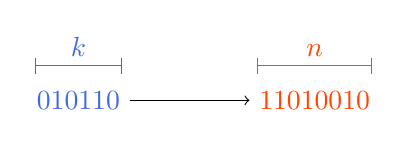
\begin{tikzpicture}
\node[RoyalBlue] (A) at (0,0) {010110};
\node[OrangeRed] (B) at (3,0) {11010010};
\draw[|-|,RoyalBlue] ($(A.north west)+(1mm,2mm)$) -- ($(A.north east)+(-1mm,2mm)$) node[midway,anchor=south] {$k$};
\draw[|-|,OrangeRed] ($(B.north west)+(1mm,2mm)$) -- ($(B.north east)+(-1mm,2mm)$) node[midway,anchor=south] {$n$};
\draw[->] (A) -- (B);
\end{tikzpicture}
\end{document}